\tikzset{>=latex} % for LaTeX arrow head
\colorlet{Ecol}{orange!90!black}
\colorlet{EcolFL}{orange!90!black}
\colorlet{veccol}{green!45!black}
\colorlet{Bcol}{violet!90}
\colorlet{Bcol1}{violet!80!blue!90}
\colorlet{Bcol2}{violet!80!red!90}
\colorlet{BFcol}{red!60!black}
\colorlet{veccol}{green!45!black}
\colorlet{Icol}{blue!70!black}
\tikzstyle{BField}=[->,thick,Bcol]
\tikzstyle{current}=[->,Icol,thick]
\tikzstyle{force}=[->,thick,BFcol]
\tikzstyle{vector}=[->,thick,veccol]
\colorlet{pluscol}{red!60!black}
\colorlet{minuscol}{blue!60!black}
\tikzstyle{charge+}=[very thin,draw=black,top color=red!50,bottom color=red!90!black,shading angle=20,circle,inner sep=0.3]
\tikzstyle{charge-}=[very thin,draw=black,top color=blue!50,bottom color=blue!80,shading angle=20,circle,inner sep=0.3]
\tikzstyle{metal}=[top color=black!15,bottom color=black!25,middle color=black!20,shading angle=10]
\tikzstyle{light metal}=[top color=black!10,bottom color=black!15,middle color=black!6,shading angle=10]
\tikzset{
  EFieldLine/.style={thick,EcolFL,decoration={markings,mark=at position #1 with {\arrow{latex}}},
                     postaction={decorate}},
  EFieldLine/.default=0.5,
  BFieldLine/.style={thick,Bcol,decoration={markings,mark=at position #1 with {\arrow{latex}}},
                                 postaction={decorate}},
  BFieldLine/.default=0.5,
  pics/Bin/.style={
    code={
      \def\R{0.12}
      \draw[pic actions,line width=0.6,#1,fill=white] % ,thick
        (0,0) circle (\R) (-135:.75*\R) -- (45:.75*\R) (-45:.75*\R) -- (135:.75*\R);
  }},
  pics/Bout/.style={
    code={
      \def\R{0.12}
      \draw[pic actions,line width=0.6,#1,fill=white] (0,0) circle (\R);
      \fill[pic actions,#1] (0,0) circle (0.3*\R);
  }},
  pics/Bin/.default=Bcol,
  pics/Bout/.default=Bcol,
  pics/magnet/.style={ %args={#1}
    code={
      \def\h{0.9}
      \coordinate (-N) at (0,\h);
      \coordinate (-S) at (0,-\h);
      \draw[pic actions,thick,top color=red!60,bottom color=red!90,shading angle=20]
        (-0.8*\h/2,0) rectangle ++(0.8*\h,\h);
      \draw[pic actions,thick,top color=blue!60,bottom color=blue!90,shading angle=20]
        (-0.8*\h/2,0) rectangle ++(0.8*\h,-\h);
      \node[pic actions] at (0, \h/2) {\textbf{N}};
      \node[pic actions] at (0,-\h/2) {\textbf{S}};
  }},
}
\tikzstyle{measure}=[<->,fill=white,midway,outer sep=0]
\contourlength{1.5pt}

% FLUX-CHANGING LOOP







% LOOP ENTERING B FIELD


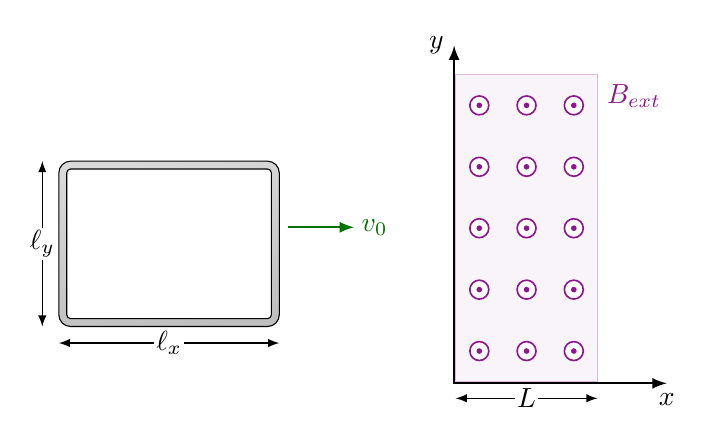
\begin{tikzpicture}
  \def\NBx{3}  % number of B field columns
  \def\NBy{5}  % number of B field rows
  \def\Lx{1.8} % B field width
  \def\Ly{3.9} % B field height
  \def\lx{2.8} % loop width
  \def\ly{2.1} % loop height
  \def\t{0.1}  % loop thickness
  
  % LOOP
  \begin{scope}[shift={(-1.8*\lx,0.18*\Ly)}]
    \draw[metal,rounded corners=1.5*\t cm,even odd rule]
      (0,0) rectangle (\lx,\ly)
      {[rounded corners=0.5*\t cm] (\t,\t) rectangle (\lx-\t,\ly-\t)};
    \draw[vector] (\lx+1.1*\t,0.6*\ly) --++ (0.3*\lx,0) node[right=-1] {$\vb{v}_0$};
    \draw[<->] (0,-2.1*\t) --++ (\lx,0) node[midway,fill=white,inner sep=0.8] {$\ell_x$}; %{\contour{white}{$\ell_x$}};
    \draw[<->] (-2.1*\t,0) --++ (0,\ly) node[midway,fill=white,inner sep=0.8] {$\ell_y$}; %{\contour{white}{$\ell_y$}};
  \end{scope}
  
  % MAGNETIC FIELDLINES
  \draw[Bcol!30,fill=Bcol!5] (0,0) rectangle (\Lx,\Ly);
  \foreach \i [evaluate={\y=(\i-0.5)*\Ly/\NBy}] in {1,...,\NBy}{
    \foreach \j [evaluate={\x=(\j-0.5)*\Lx/\NBx}] in {1,...,\NBx}{
      \pic[scale=1] at (\x,\y) {Bout};
    }
  }
  \node[Bcol,below right] at (\Lx,\Ly) {$\vb{B}_\text{ext}$};
  
  % AXES
  \draw[<->,thick,shift={(-0.02,-0.02)}]
    (0,1.1*\Ly) node[left] {$y$} -- (0,0) -- (1.5*\Lx,0) node[below] {$x$};
  \draw[<->] (0,-2.1*\t) --++ (\Lx,0) node[midway,fill=white,inner sep=0.8] {$L$};
  
\end{tikzpicture}
